\documentclass{article}
% Chinese
% \documentclass[UTF8, nofonts, mathptmx, 12pt, onecolumn]{article}
% \usepackage{xeCJK}
% \setCJKmainfont{SimSun}
\usepackage{amsmath}
\usepackage{amsfonts}
\usepackage{amssymb}
\usepackage{wasysym}
% \usepackage{ctex}
\usepackage{graphicx}
\usepackage{float}
\usepackage{geometry}
\geometry{a4paper,scale=0.8}
\usepackage{caption}
\usepackage{subcaption}
% \newcommand{\oiint}{\mathop{{\int\!\!\!\!\!\int}\mkern-21mu \bigcirc} {}}
\newcommand*{\dif}{\mathop{}\!\mathrm{d}}
\newcommand*{\md}{\mathop{}\!\mathrm{d}}
\newcommand*{\me}{\mathrm{e}}

\usepackage{parskip}
\setlength{\parindent}{0cm}

\usepackage{bm}
\let\Oldmathbf\mathbf
\renewcommand{\mathbf}[1]{\boldsymbol{\Oldmathbf{#1}}}
\let\eqnarray\align

\author{Xiping Hu}
\usepackage{authblk}
\author{Xiping Hu}
\affil{http://thehxp.tech/}
\title{Homework for Analogue Electronics}

\begin{document}
\maketitle

\begin{figure}[H]
  \centering
  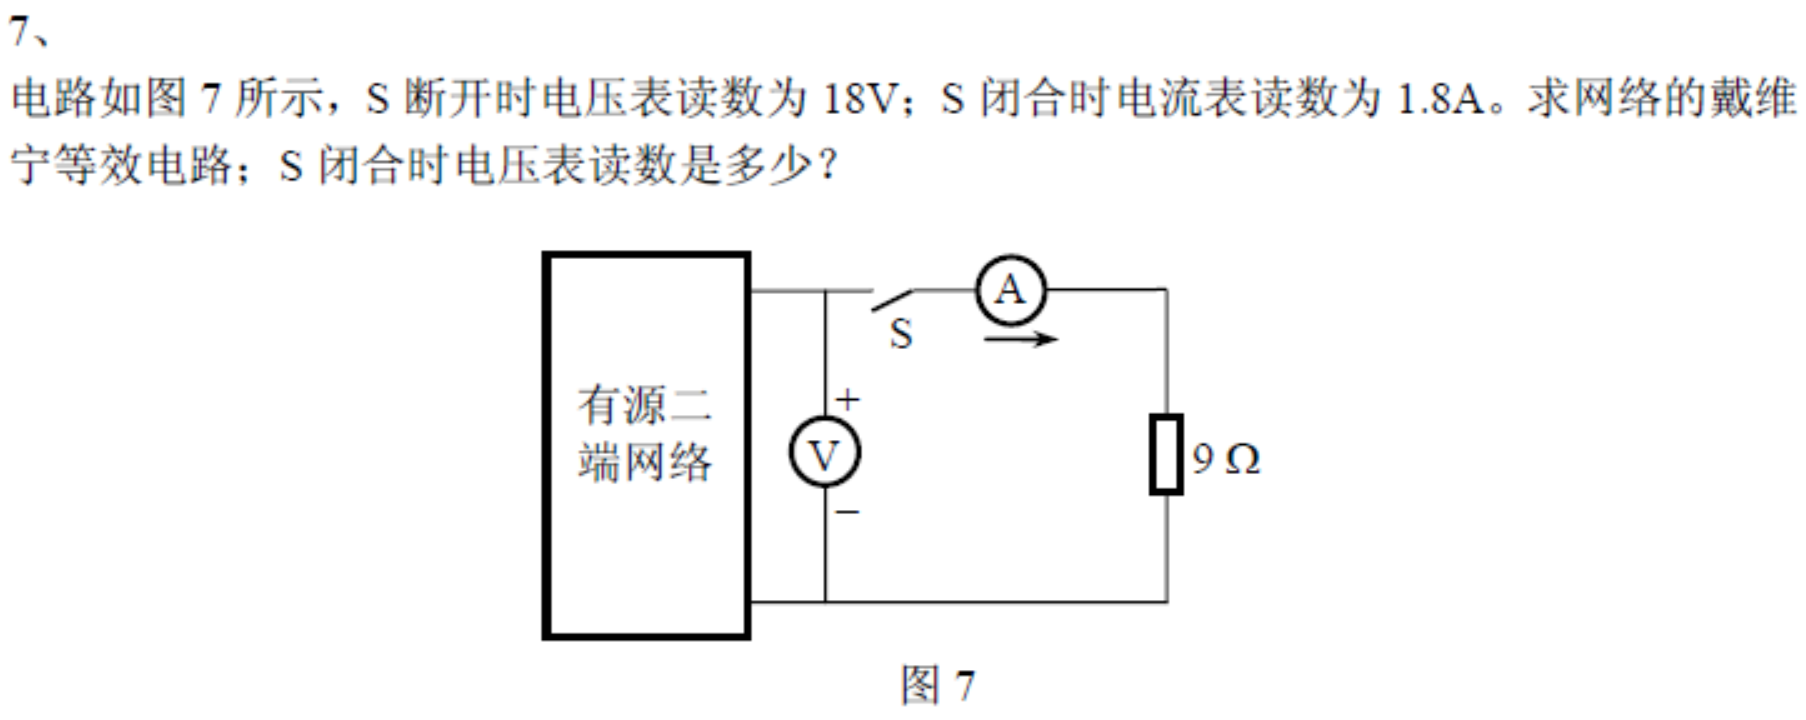
\includegraphics[width=\linewidth]{figures/7}
  \label{fig:}
\end{figure}

\paragraph{Solution}

When $S$ is closed, we can calculate the inner resistance of the notwork to the left.

\begin{equation*}
  \begin{aligned}
    R = \dfrac{18 \  \mathrm{V}}{1.8 \  \mathrm{A}} - 9 \  \mathrm{\Omega} = 1 \  \mathrm{\Omega}
  \end{aligned}
\end{equation*}

So that the whole circuit is equivalent to this circuit below

\begin{figure}[H]
  \centering
  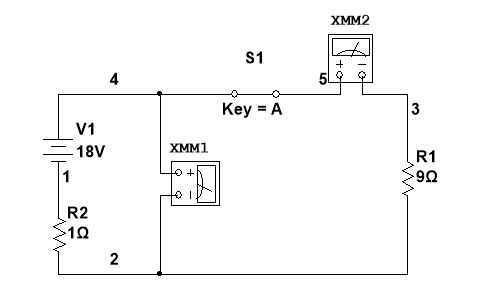
\includegraphics[width=0.5\linewidth]{figures/10}
  \label{fig:}
\end{figure}

\begin{equation*}
  \begin{aligned}
    U = \dfrac{18 \  \mathrm{V}}{10 \  \mathrm{\Omega}} \times 9 \  \mathrm{\Omega} = 16.2 \  \mathrm{V}
  \end{aligned}
\end{equation*}




\end{document}